% Fig 2.3 — Taxonomy of query-enhancement techniques.
%
% REDESIGN (not a restore) of archive/system_diagrams_dropped/fig_2_2_qe_taxonomy.tex,
% 2026-08-09. Renamed 2_2 -> 2_3 to match the printed number (chapter2.tex order: taxonomy, then placement).
%
% WHY A REDESIGN. The archived figure split QE into "lexical/statistical" vs
% "LLM-based generative". §2.1.4 was since rewritten around Song and Zheng's FOUR
% atomic operations — expansion, decomposition, disambiguation, abstraction
% (chapter2.tex:84, \cite{song_2024_a}), each with its own \subsubsection. Restoring
% the old figure would have put a figure and its own section in contradiction.
%
% Osman's edit carried forward (FIGURE_NOTES_MOHAMMED.md §2): the in-image
% "built on in this thesis" annotation is deleted; it is stated in the caption.
%
% Every leaf matches a technique named in chapter2.tex:86-104 and §2.5.
\documentclass[border=4pt]{standalone}
\usepackage{tikz}
% Shared TikZ style for thesis figures.
% Each fig_*.tex \input{} this file after \usepackage{tikz}.
% Defines a muted, examiner-friendly color palette and semantic box styles.

\usepackage{xcolor}
\usepackage{fontawesome5}
\usetikzlibrary{positioning, arrows.meta, shapes.geometric, calc, fit, backgrounds}

% ─── Palette ───────────────────────────────────────────────────────────
% Each role has a stroke color (dark) and a fill color (very light).
% Designed to be grayscale-safe — lightness differs enough that B&W printing
% still preserves the distinction.

\definecolor{thQueryS}{HTML}{4A6FA5}    \definecolor{thQueryF}{HTML}{E8EEF6}   % query / input
\definecolor{thLLMS}{HTML}{6D4A8F}      \definecolor{thLLMF}{HTML}{ECE5F2}     % LLM / generation
\definecolor{thRetS}{HTML}{3D7A4F}      \definecolor{thRetF}{HTML}{E4EFE7}     % retriever
\definecolor{thDataS}{HTML}{6A6A6A}     \definecolor{thDataF}{HTML}{F1F1F1}    % corpus / data
\definecolor{thFusionS}{HTML}{A05A30}   \definecolor{thFusionF}{HTML}{F4E8DF}  % fusion
\definecolor{thOutS}{HTML}{1F6F8A}      \definecolor{thOutF}{HTML}{DEEAEF}     % output / final
\definecolor{thHiS}{HTML}{0D4D63}       \definecolor{thHiF}{HTML}{C8D9DF}      % highlighted (our contribution)
\definecolor{thMuted}{HTML}{5C5C5C}

% ─── Box styles ────────────────────────────────────────────────────────
% Usage in tikzpicture options:  query/.style={thQuery}, llm/.style={thLLM}, ...
% Or directly on nodes:          \node[thLLM] (m) {...};
\tikzset{
  thBase/.style={rectangle, draw, rounded corners=2pt,
                 minimum width=28mm, minimum height=10mm,
                 align=center, font=\small, line width=0.6pt,
                 inner sep=4pt},
  thQuery/.style={thBase, draw=thQueryS, fill=thQueryF},
  thLLM/.style={thBase, draw=thLLMS, fill=thLLMF},
  thRet/.style={thBase, draw=thRetS, fill=thRetF},
  thData/.style={cylinder, shape border rotate=90, aspect=0.3, draw=thDataS, fill=thDataF,
                 minimum width=24mm, minimum height=12mm, align=center, font=\small, line width=0.6pt},
  thFusion/.style={thBase, draw=thFusionS, fill=thFusionF},
  thOut/.style={thBase, draw=thOutS, fill=thOutF},
  thHi/.style={thBase, draw=thHiS, fill=thHiF, line width=1pt},
  thArrow/.style={-{Stealth[length=2.5mm]}, line width=0.7pt, draw=thMuted},
  thLabel/.style={font=\footnotesize\itshape, color=thMuted},
  thStage/.style={font=\bfseries\footnotesize, color=thMuted},
}

% ─── Icon helpers ──────────────────────────────────────────────────────
% Tiny FontAwesome icons that can sit inside a node prefix.
% Usage:  \node[thQuery] {\thIconQuery~User query};
\newcommand{\thIconQuery}{\textcolor{thQueryS}{\faSearch}}
\newcommand{\thIconUser}{\textcolor{thQueryS}{\faUser}}
\newcommand{\thIconLLM}{\textcolor{thLLMS}{\faBrain}}
\newcommand{\thIconRet}{\textcolor{thRetS}{\faNetworkWired}}
\newcommand{\thIconCorpus}{\textcolor{thDataS}{\faDatabase}}
\newcommand{\thIconFusion}{\textcolor{thFusionS}{\faCodeBranch}}
\newcommand{\thIconOut}{\textcolor{thOutS}{\faFile}}
\newcommand{\thIconEval}{\textcolor{thOutS}{\faChartBar}}
\newcommand{\thIconStar}{\textcolor{thHiS}{\faStar}}
\newcommand{\thIconCog}{\textcolor{thMuted}{\faCog}}


\begin{document}
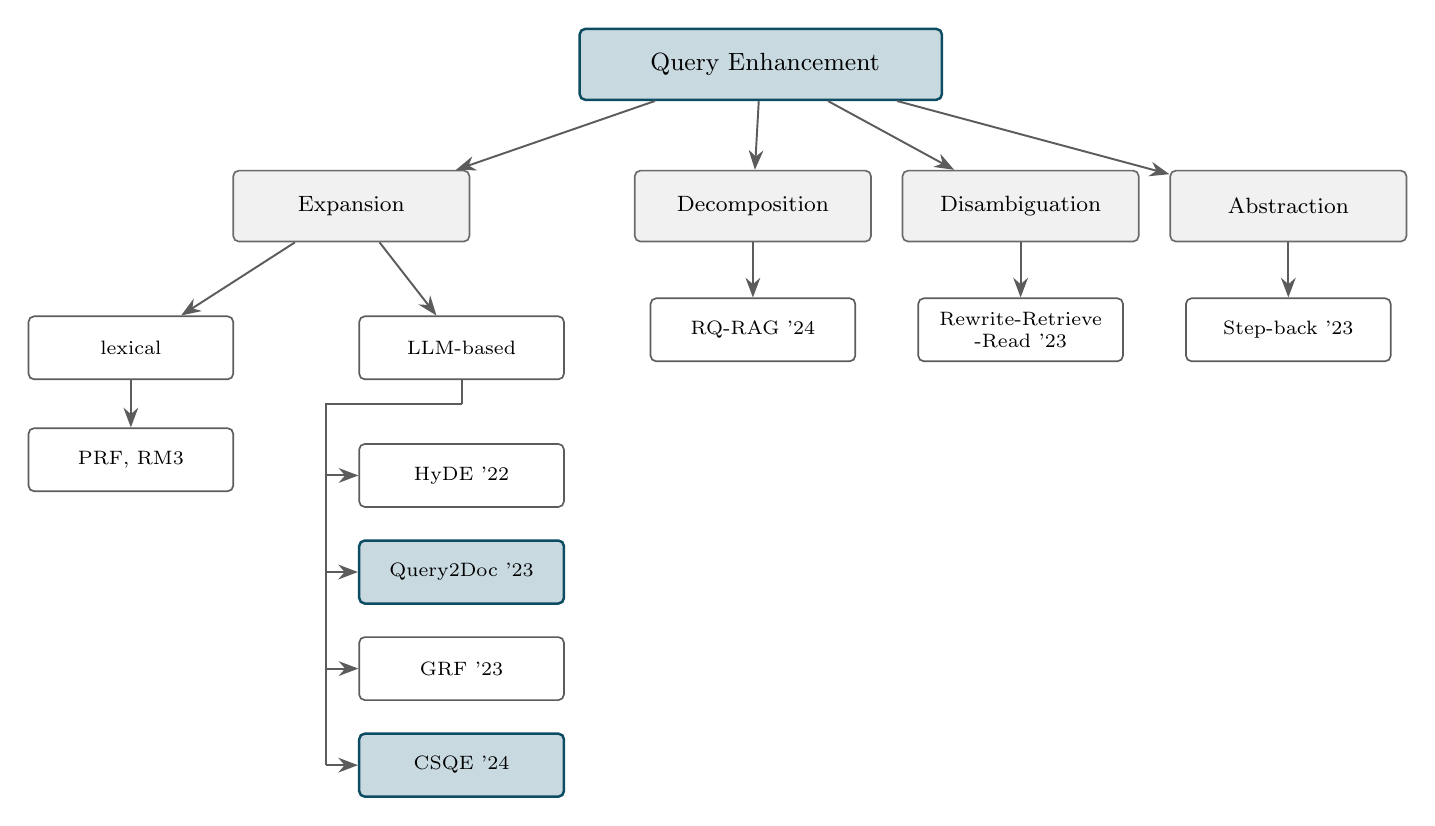
\begin{tikzpicture}[
    root/.style={thBase, draw=thHiS, fill=thHiF, minimum width=46mm,
                 minimum height=9mm, line width=0.9pt, font=\small},
    family/.style={thBase, fill=thDataF, draw=thDataS, minimum width=30mm,
                   minimum height=9mm, font=\footnotesize},
    sub/.style={thBase, fill=white, draw=thMuted, minimum width=26mm,
                minimum height=8mm, font=\scriptsize},
    leaf/.style={thBase, fill=white, draw=thMuted, minimum width=26mm,
                 minimum height=8mm, font=\scriptsize},
    ours/.style={thBase, draw=thHiS, fill=thHiF, minimum width=26mm,
                 minimum height=8mm, line width=0.9pt, font=\scriptsize}
]

  % ─── Root ──────────────────────────────────────────────────────────────
  \node[root] (root) at (0,0) {\thIconStar~Query Enhancement};

  % ─── Four atomic operations (Song and Zheng) ───────────────────────────
  \node[family] (exp)   at (-52mm, -18mm) {Expansion};
  \node[family] (dec)   at ( -1mm, -18mm) {Decomposition};
  \node[family] (dis)   at ( 33mm, -18mm) {Disambiguation};
  \node[family] (abs)   at ( 67mm, -18mm) {Abstraction};

  \draw[thArrow] (root) -- (exp);
  \draw[thArrow] (root) -- (dec);
  \draw[thArrow] (root) -- (dis);
  \draw[thArrow] (root) -- (abs);

  % Single representative technique under the three non-expansion families
  \node[leaf, below=7mm of dec] (rqrag)   {RQ-RAG '24};
  \node[leaf, below=7mm of dis] (rewrite) {Rewrite-Retrieve\\-Read '23};
  \node[leaf, below=7mm of abs] (stepback){Step-back '23};
  \draw[thArrow] (dec) -- (rqrag);
  \draw[thArrow] (dis) -- (rewrite);
  \draw[thArrow] (abs) -- (stepback);

  % ─── Expansion splits again: lexical vs LLM-based ──────────────────────
  \node[sub] (lex) at (-80mm, -36mm) {lexical};
  \node[sub] (gen) at (-38mm, -36mm) {LLM-based};
  \draw[thArrow] (exp) -- (lex);
  \draw[thArrow] (exp) -- (gen);

  \node[leaf, below=6mm of lex] (prf) {PRF, RM3};
  \draw[thArrow] (lex) -- (prf);

  % The four LLM-based techniques are SIBLINGS, not a chain. Chaining them
  % hyde -> q2d -> grf -> csqe would read as "HyDE is the parent of Query2Doc",
  % which is false. They hang off a shared spine, the standard tree idiom.
  \node[leaf,  below=8mm of gen]      (hyde) {HyDE '22};
  \node[ours,  below=4mm of hyde]     (q2d)  {Query2Doc '23};
  \node[leaf,  below=4mm of q2d]      (grf)  {GRF '23};
  \node[ours,  below=4mm of grf]      (csqe) {CSQE '24};

  \coordinate (spine) at ($(gen.south)+(0,-3mm)$);
  \draw[thArrow, -] (gen.south) -- (spine);
  \draw[thArrow, -] (spine) -- ($(spine -| csqe.west)+(-4mm,0)$)
                    -- ($(csqe.west)+(-4mm,0)$);
  \foreach \n in {hyde,q2d,grf,csqe}{%
    \draw[thArrow] ($(\n.west)+(-4mm,0)$) -- (\n.west);}

\end{tikzpicture}
\end{document}
